% Lines that start with a % are comments and are not included when the LaTeX file is converted to a pdf

% Set up the document class - this can be changed if a different format is required 
\documentclass[12pt,a4paper]{article}

% Include packages that contain additional features, for example including special mathematical characters and images in your document
\usepackage{amssymb,amsmath,graphicx}


\usepackage{geometry}
 \geometry{
 a4paper,
 total={170mm,257mm},
 left=20mm,
 top=20mm,
 }



% The beginning of the document...
\begin{document}

% Please change the following accordingly...
\centerline{\large Exercise sheet 2}\vspace{0.5em}
\centerline{\large by Maximilian Richter and Christian Heppe}\vspace{1em}

% Split the different exercises into different sections...
\section*{Exercise 2)}

% To include a plot it must be in the same directory as the .tex file.
a) Trajectories of the three masses for different values for stepsize $h$\\
% Remove the "%" in the following line and change the "plot.png" to the name of the plot to include.
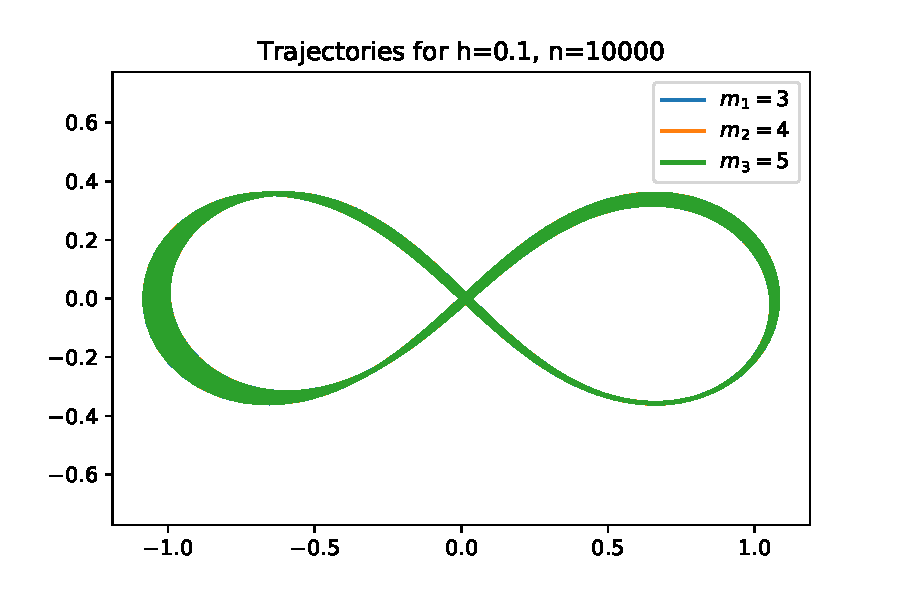
\includegraphics[width=8cm]{a_h_1.pdf}
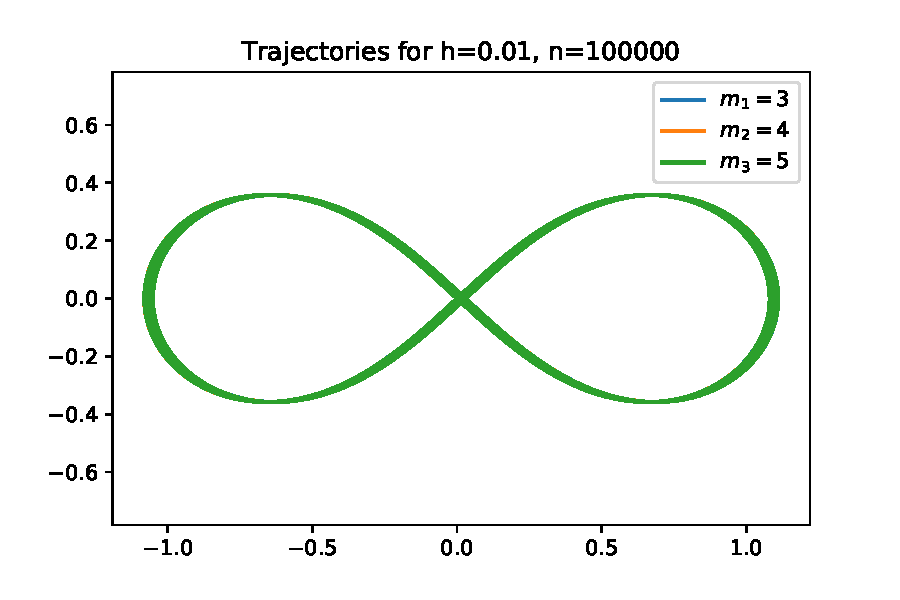
\includegraphics[width=8cm]{a_h_01.pdf}\\
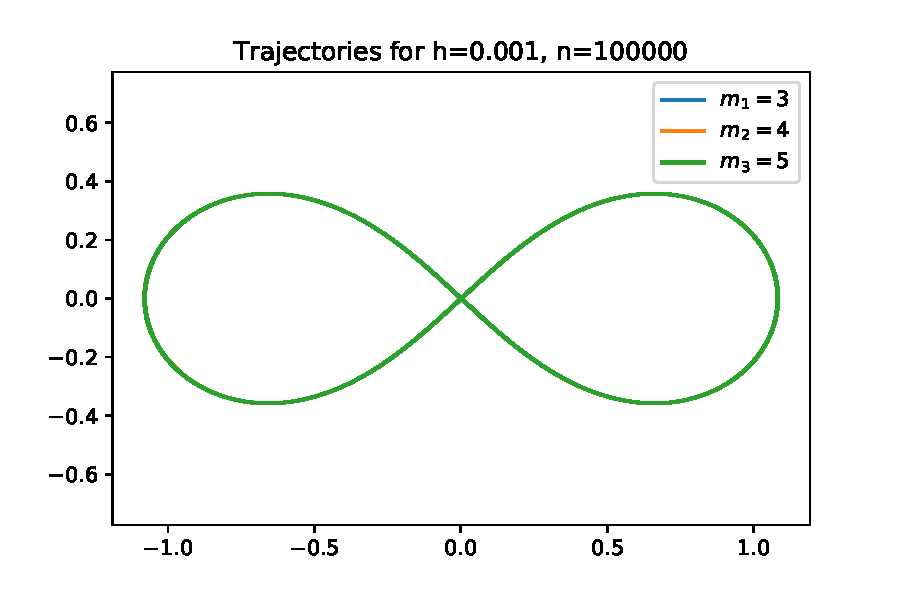
\includegraphics[width=8cm]{a_h_001.pdf}
\newline
As one can see, after multiple periods, the orbits changes its shape for big values of $h$. The smaller one sets $h$, the more precise the orbit of the bodies will stay over time\\
\newline
b) Meissel-Burrau problem\\
\newline
We observe that for a minimum value of h=0.0001 we can obtain reliable estimates for the time of the first five closest encounters of the three masses.\\
For a better understanding of the shown trajectories we added a GIF-file into the ZIP-archive showing the movement of the three masses for the last configuration as a short animation 
For further details see the python-code in the appendix.\\
\newpage
i) Trajectories on the orbital plane\\
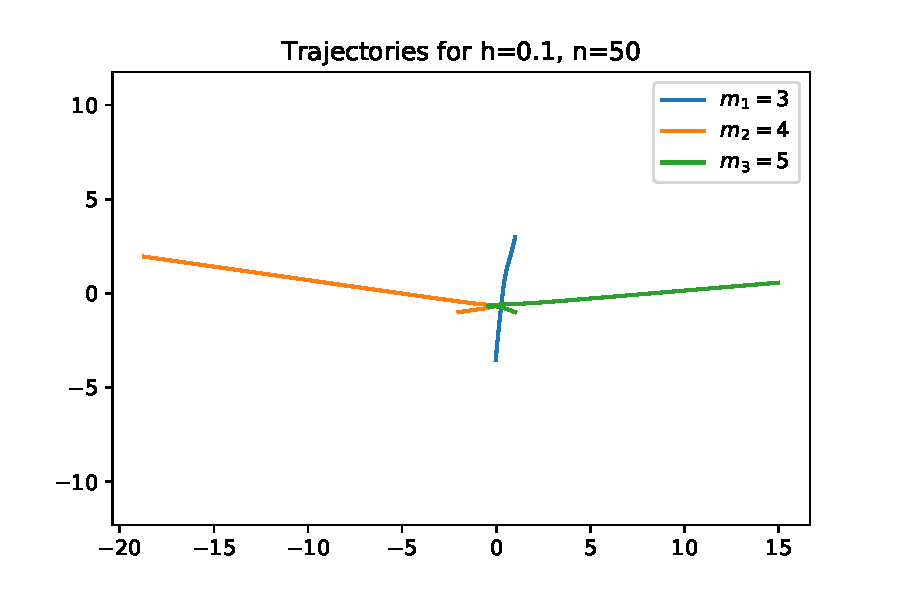
\includegraphics[width=8cm]{b_h_1.pdf}
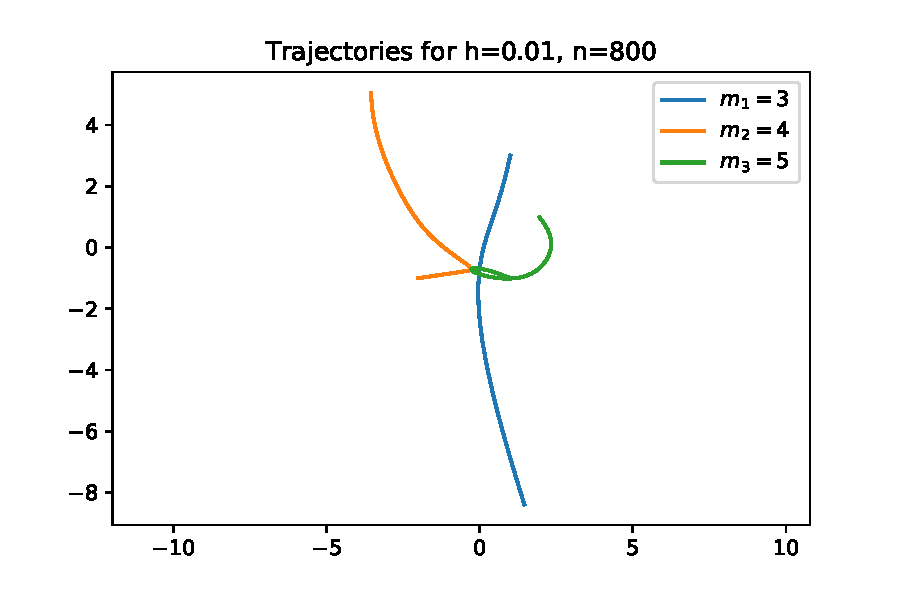
\includegraphics[width=8cm]{b_h_01.pdf}\\
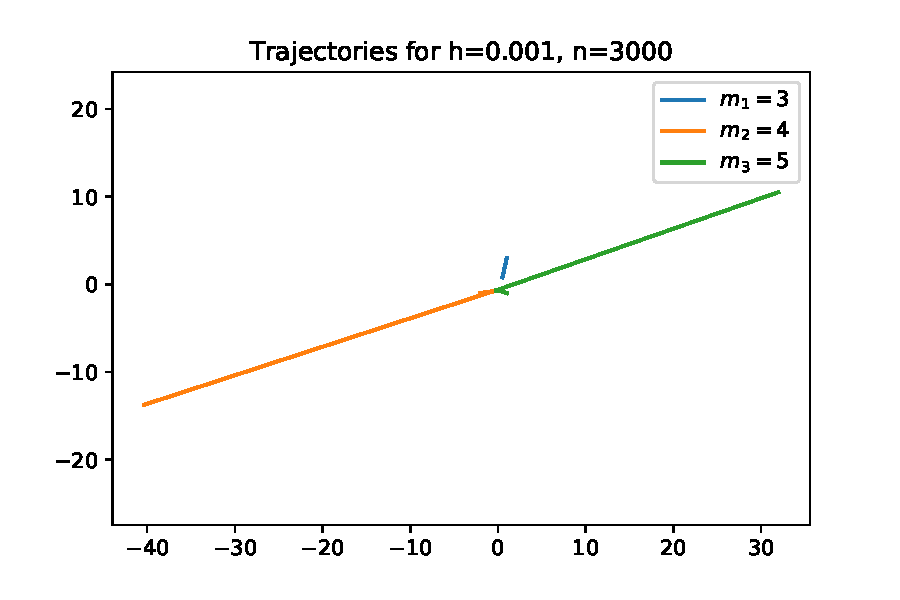
\includegraphics[width=8cm]{b_h_001.pdf}
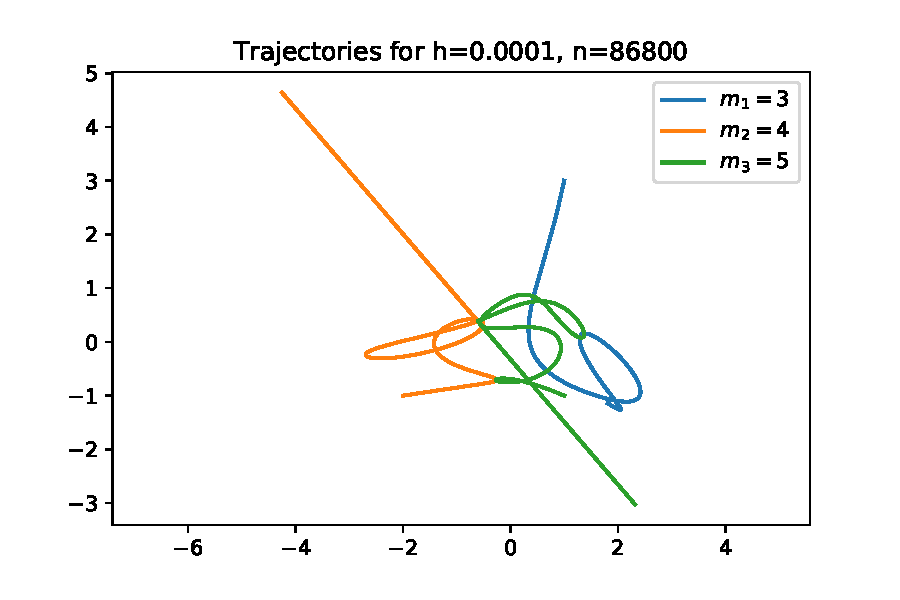
\includegraphics[width=8cm]{b_h_0001.pdf}\\
ii) Relative distances of the bodies\\
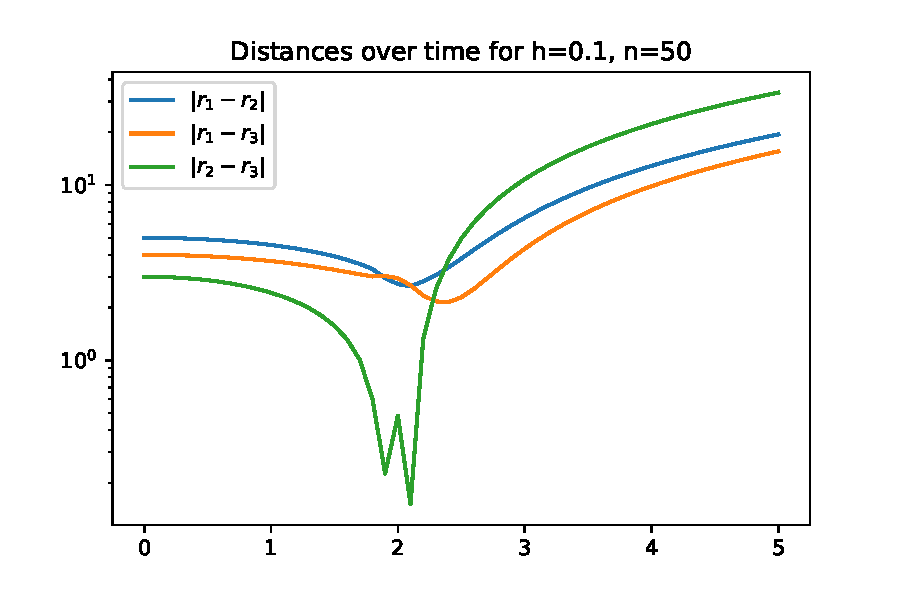
\includegraphics[width=8cm]{dist_h_1.pdf}
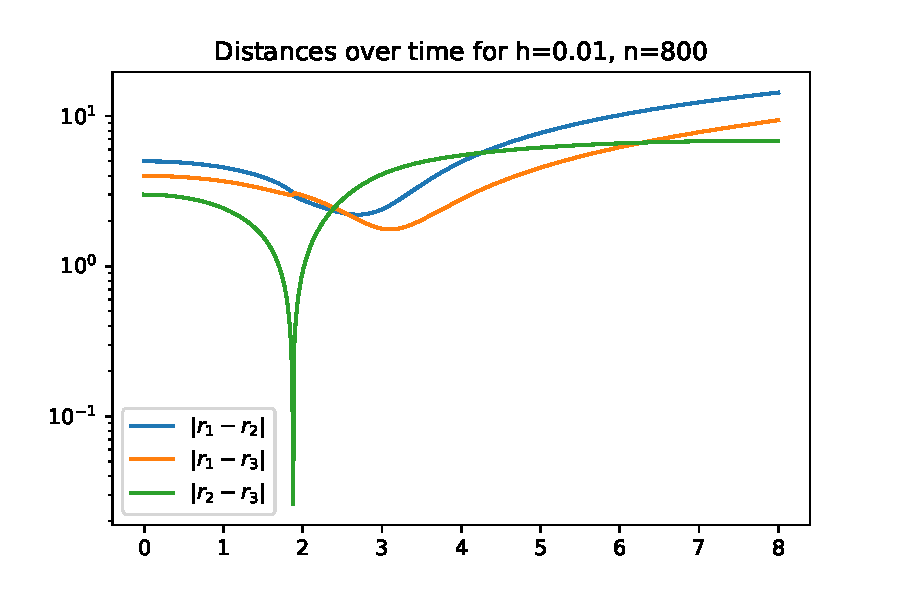
\includegraphics[width=8cm]{dist_h_01.pdf}\\
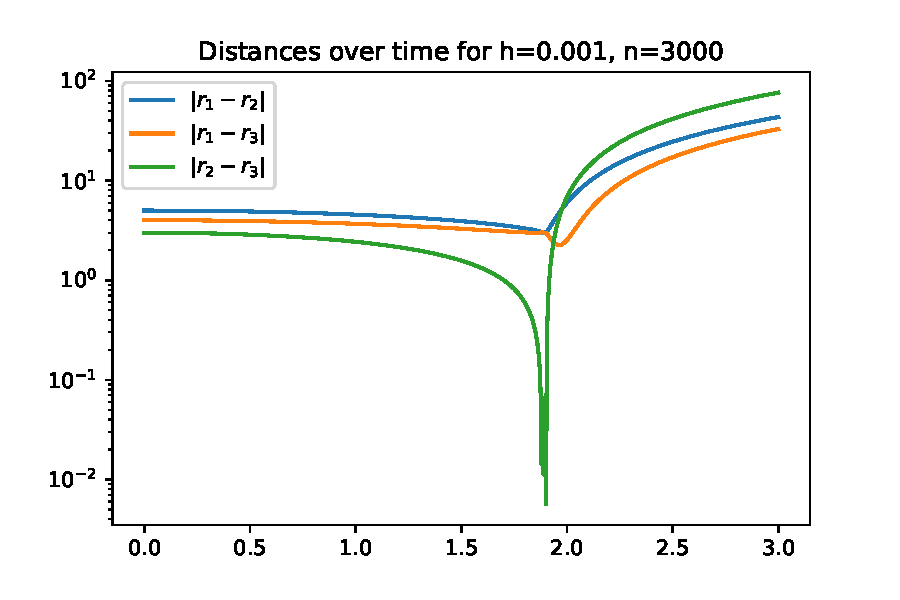
\includegraphics[width=8cm]{dist_h_001.pdf}
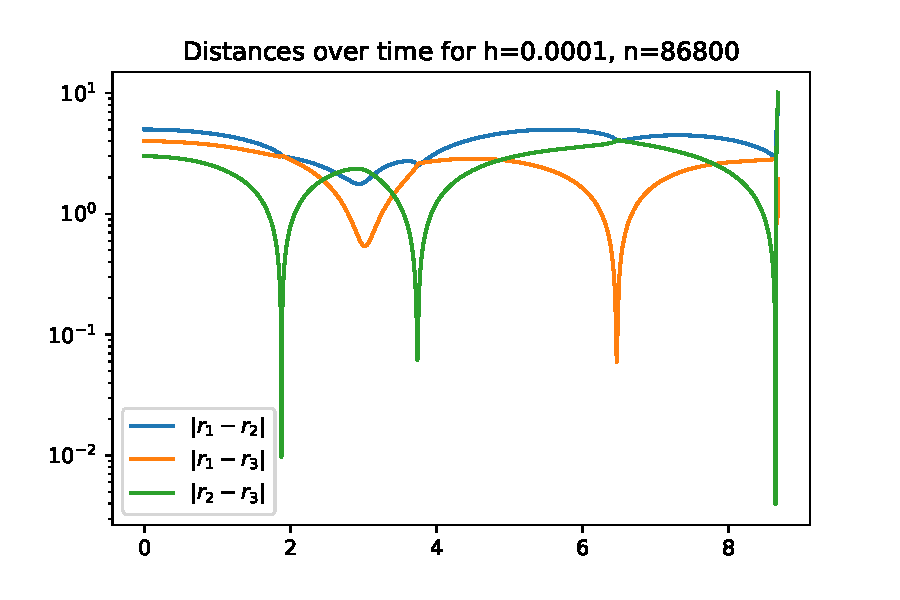
\includegraphics[width=8cm]{dist_h_0001.pdf}\\
\newpage
iii) Total Energy \\
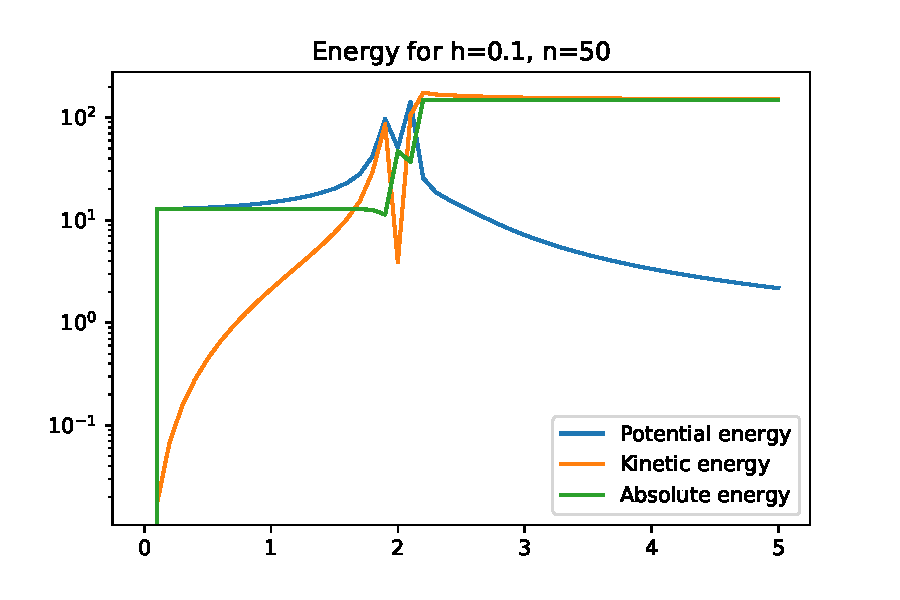
\includegraphics[width=8cm]{energ_h_1.pdf}
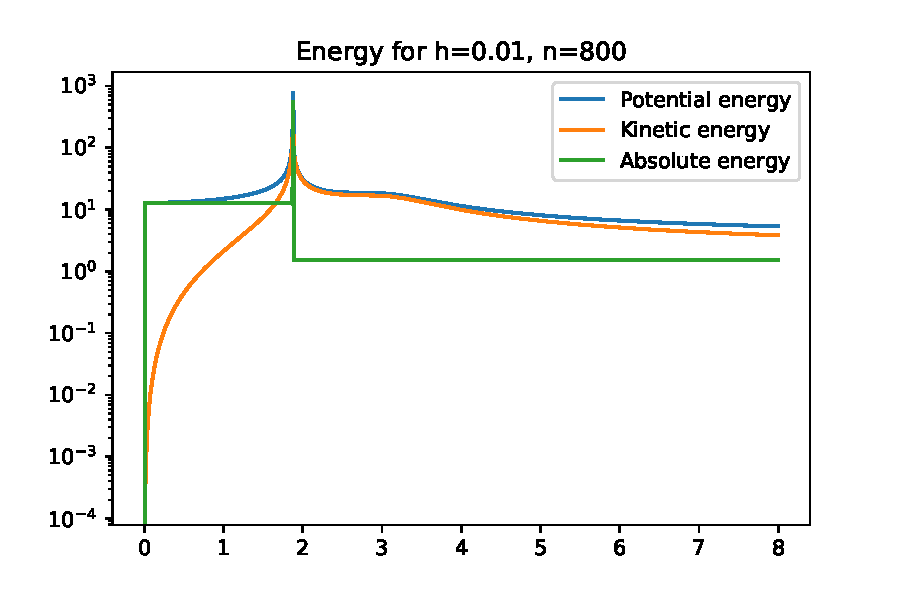
\includegraphics[width=8cm]{energ_h_01.pdf}\\
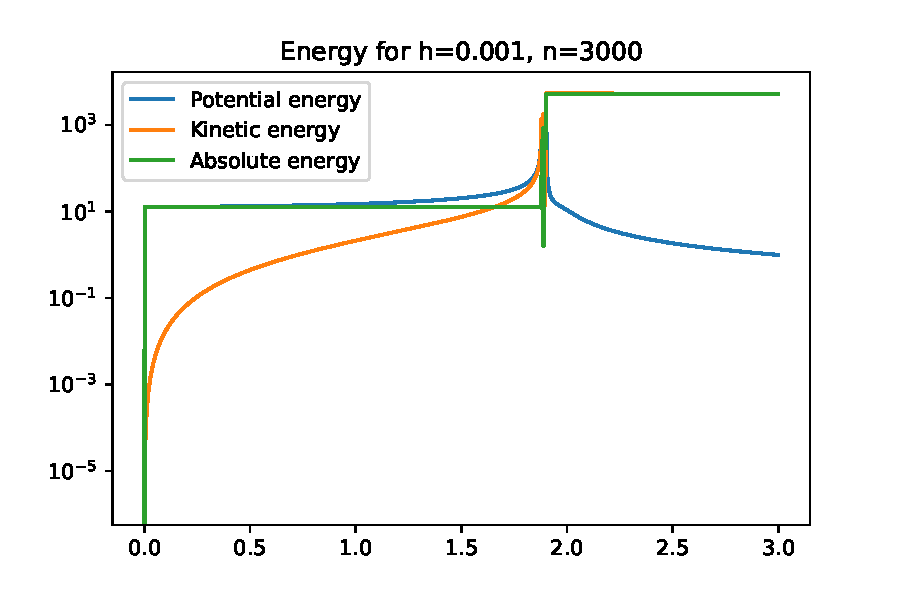
\includegraphics[width=8cm]{energ_h_001.pdf}
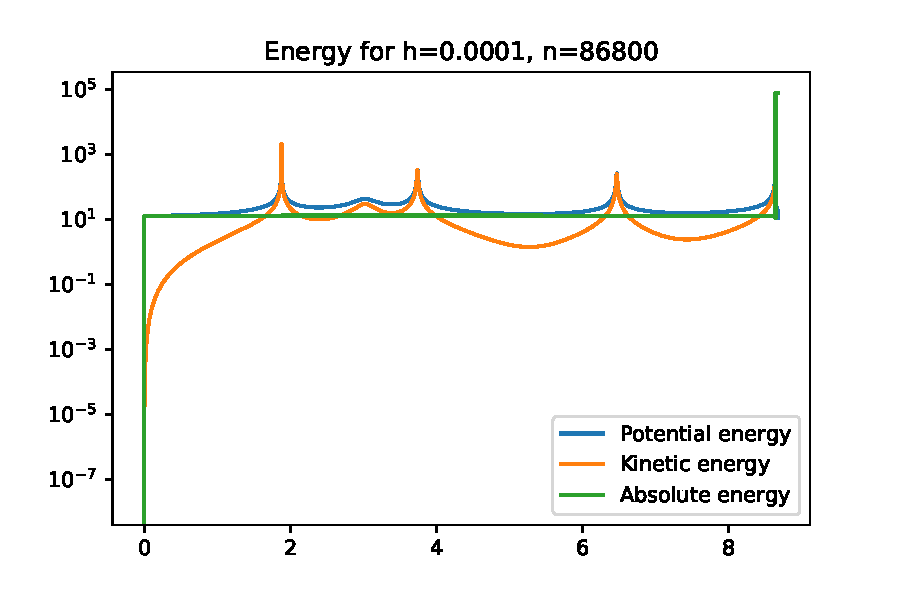
\includegraphics[width=8cm]{energ_h_0001.pdf}\\
\end{document}

